% ==============================================================================
\chapter{Thin sensors studies}
\label{ch:ThinSensorsStudies}
%==============================================================================    

\section{Samples and sensors geometries}
Operating conditions for the Timepix3 readout ASICs:
\begin{itemize}
\item I\textsubscript{krum} DAC is set to 10.
\item TOT clock frequency: $40\,\megahertz$
\item VFBK: 150
\end{itemize}
 
\section{Test-beam setup}
\subsection{EUDET telescope ?} 
\subsection{The Timepix3 telescope} \label{sec:Timepix3Telescope}
The Timepix3 telescope is used as a beam reference telescope and is
shown in Figure~\ref{fig:TPX3Telescope}. The telescope is used to
reconstruct the tracks of the particles going through its planes and
extrapolate the position on the Device Under Test (DUT). This allows
to compare the position of the hit on the DUT with the reconstructed
track and calculate the position, time resolutions and the efficiency
of the device. The Timepix3 telescope is made of 6 planes of Timepix3
ASICs~\cite{Timepix3_Poikela} bump bonded to $300\,\micron$ thick
p-in-n planar sensors. The planes are rotated by $9\degrees$ around
the x axis (perpendicular to the beam axis) and the z axis (parallel
to the beam axis) to optimise the charge sharing within the sensors
and obtain a pointing resolution of $\sim$$2\,\micron$ on the device
under test (DUT). The data-driven zero-suppressed mode is used for the
data acquisition of the Timepix3 readout ASICs.

\begin{figure}[htbp]
  \centering
  \begin{tikzpicture}
    \node[anchor=south west,inner sep=0] (image) at
    (0,0){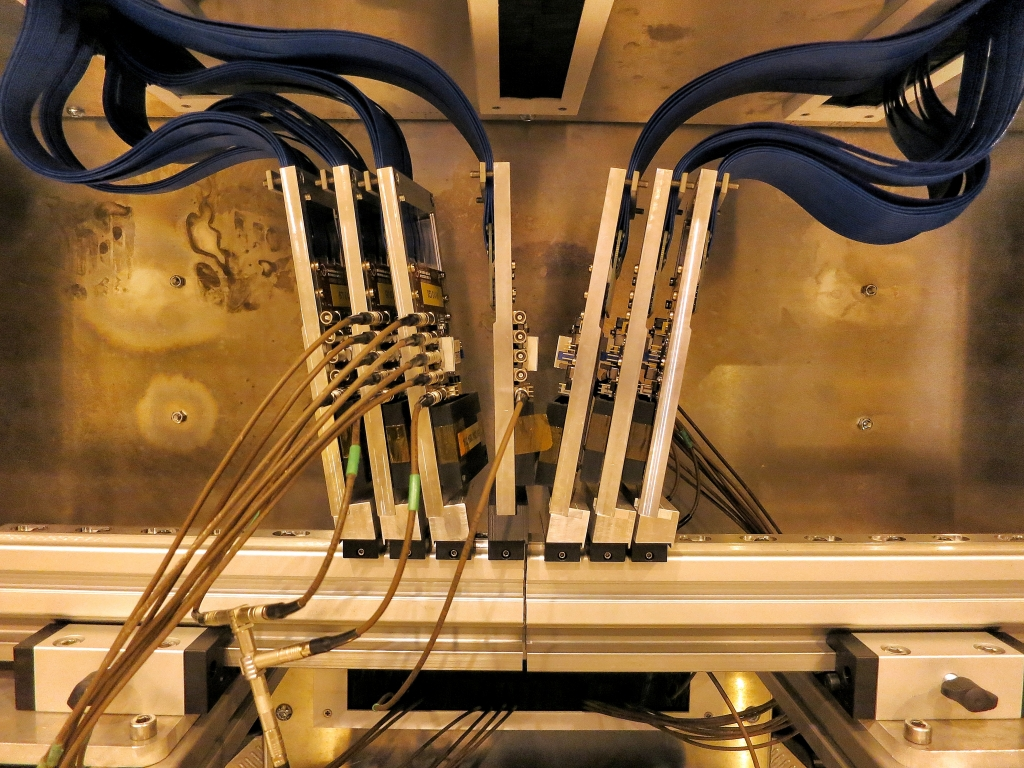
\includegraphics[width=0.6\textwidth]{ActiveEdge/Timepix3Telescope.jpeg}};
    \begin{scope}[x={(image.south east)},y={(image.north west)}]
      \node[above, color=white] at (0.5, 0.85) {Device Under Test};
      \node[above, color=white] at (0.5, 0.78) {(\textbf{DUT})};
    \end{scope}
  \end{tikzpicture} 
  \caption{The Timepix3 beam reference telescope.}
  \label{fig:TPX3Telescope}
\end{figure}

\subsection{Experimental setup at the CERN SPS}
The assemblies are tested at the H6 beam of the CERN SPS using the $120\,\gev$
pion beam. The particle rate obtained per spill is $\sim2.6 \times
10^6$ (UNITS?). The telescope planes were positioned in a way to give
the best tracking resolution for the given beam energy and the level
of multiple scatterings.
For most of the measurements, the DUT is perpendicular
to the beam. A scan was done on the bias voltage and the threshold of
the DUT. The bias scan allows to obtain the depletion voltage.

\section{Reconstruction softwares}
\subsection{EUTelescope}
The EUTelescope software~\cite{Rubinskiy} is used to reconstruct the
telescope tracks and analyse the telescope data. It is based on the
ILCSoft framework (REF?). Using a pipeline of Marlin
processors~\cite{Gaede:2006pj}, it allows to convert the raw data to a
ROOT (REF?) format and with the intermediate steps in the LCIO (REF?)
format. The reconstruction chain is defined in the steps below:

\begin{enumerate}
\item Converter: converts the raw files written by each telescope
planes and the DUT in a binary format to an LCIO event. The
data-driven zero-suppressed mode is used for the data acquisition of
the Timepix3 readout ASICs. This mode allows for a very low dead-time
and all the particles at the SPS spill are recorded. Every hit is
written with a 64-bit time-stamp (\texttt{long long int}) related to
the TOA (time-of-arrival). The hits written in the raw file are not
necessarily ordered in time. In the converter processor, the hits
within a timing window of 3~ms are read and filled into a vector. The
hits in the vector are ordered in time according to their time
stamps. An LCIO event is built by choosing the hits in the six
telescope planes and the DUT with time stamps differing by
$2.5\,\microsecond$. With this constraint, most probably one track per
event is obtained.
Hot pixels (with the maximum allowed frequency of 0.1) are as well
calculated and also the $\eta$-correction~\cite{Belau:1983eh} values.

\item Clustering: the clusters in each plane is found.
\item Hit making: reconstruction of the hit position for each cluster
with the $\eta$-correction method.
\item Alignment: by assuming straight tracks, the alignment processor
uses Millepede~II algorithm~\cite{Blobel20065} to align the telescope
planes with respect to each other. It consists of a least squares
minimisation problem ($\chi^2$minimisation). A proper definition of
the geometry is important.
\item Track finding: fits the tracks based on the hits on the
telescope planes with taking to account the multiple scatterings
(radiation length of the material for the described geometry),
positions of the planes. The \texttt{EUTelTestFitter} algorithm is used for the
analysis of the test-beam. (TO PUT SOME CHI2 DISTRIBUTION PLOTS). The
tracks are then extrapolated on the DUT.
\end{enumerate} 

\subsection{pyEudetAnalysis}
For the analysis of the DUT data, the python-based software
\texttt{pyEudetanalysis} is used. It can be found as a GitHub directory~\cite{pyeudet}.


\section{AllPix: a \textsc{Geant4}-based simulation software}
AllPix~\cite{allpix}, is used as a wrapper on \textsc{Geant4} to
simulate the test beam setup. The software is written in C/C++. It
provides a flexible interface to define the geometry of the
setup. Figure~\ref{fig:TPX3TelescopeAllpix} shows the telescope planes
and the DUT simulated in AllPix.

\begin{figure}[htbp]
  \centering
  \begin{tikzpicture}
    \node[anchor=south west,inner sep=0] (image) at
    (0,0){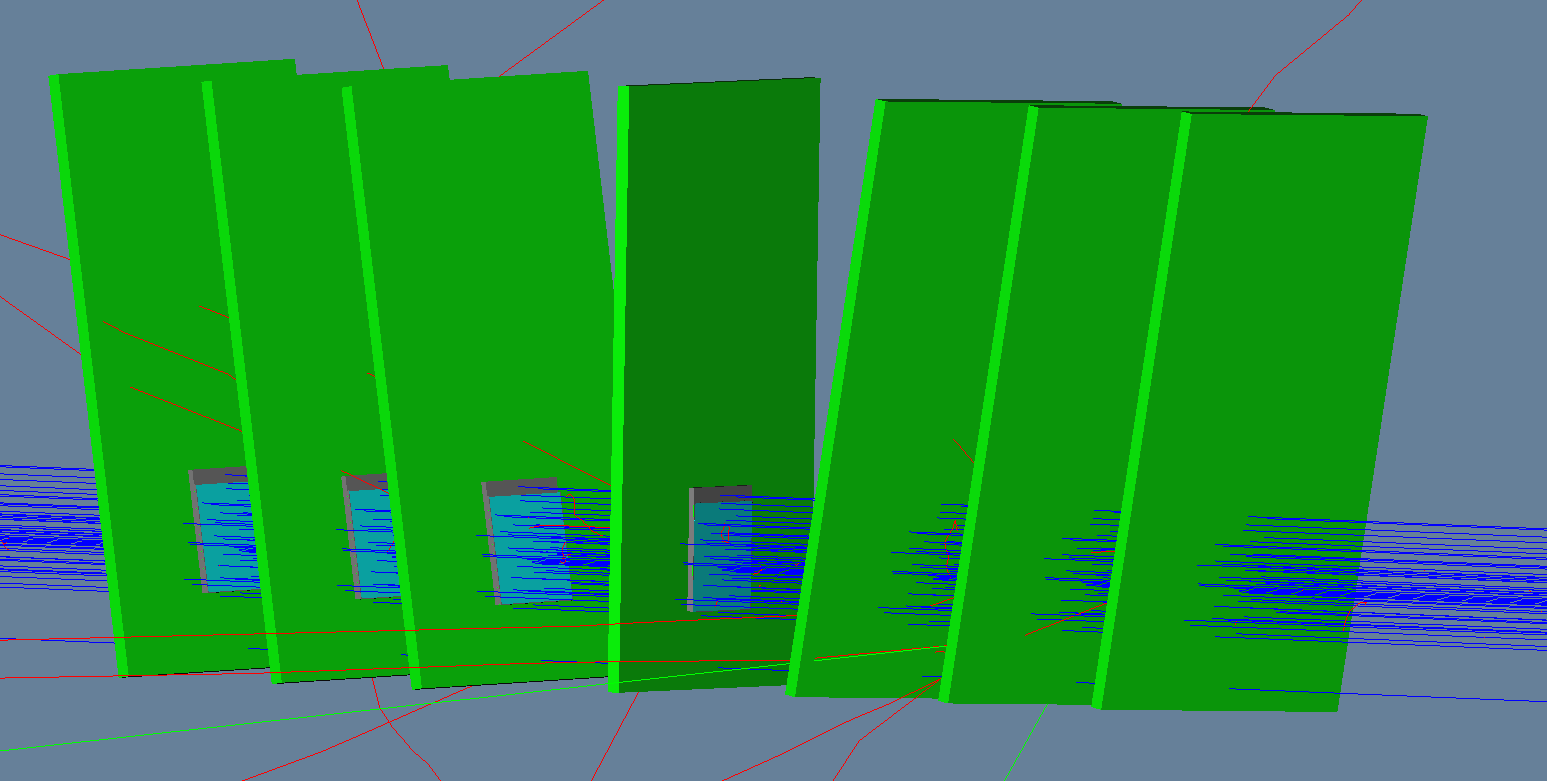
\includegraphics[width=0.8\textwidth]{figures/ActiveEdge/Allpix_telescope_withParticles.png}};
    \begin{scope}[x={(image.south east)},y={(image.north west)}]
      \node[above, color=white] at (0.45, 0.65) {\textbf{DUT}};
    \end{scope}
  \end{tikzpicture}
  \caption{Simulation of the Timepix3 telescope with AllPix.}
  \label{fig:TPX3TelescopeAllpix}
\end{figure}

The main components of the software are described here-below:
\begin{enumerate}
\item Digitiser: \textsc{Geant4}, for each simulation step
  (\texttt{G4Step}) through the matter, provides the energy deposited
  in the sensitive material. The step length can be customised. For
  thin sensors simulations a step of $2\,\micron$ is selected and
  provides a precise energy deposition. The semiconductor physics in a
  Silicon detector is then defined in the digitiser. The drift and
  diffusion are performed at each step to simulate the electron-hole
  pair movement in the electric and magnetic fields. The readout ASIC
  is also simulated in the digitiser. The electronic noise is added
  and a threshold is applied to the hits. The hit energy is converted to the
  digital value TOT (time-over-threshold) using the readout ASICs calibrations.
\item \texttt{pixeldetector.xml}: defines a pixel detector
(\texttt{<pixeldet id=''300"/>}) with a unique ID. It contains all the
properties of the pixel detector like the pixel pitch, detector
thickness, chip thickness, PCB properties and other geometry
properties related to an assembly. It can be customised and define the
parameters of the digitisers. This will allow to run the program
without needing to compile whenever one wants to change a parameter.
\item \texttt{macro.in}: Define the position of the detectors in the
space by giving the x, y and z position of the centre of the detectors
and the rotations around the x, y and z axes. The physics list used by
\textsc{Geant4} is also defined in this file. Visualisation parameters
are also given. The General Particle Source (GPS), which is the
\textsc{Geant4} toolkit for Monte-Carlo of the high-energy particle
transport is also described in the macro. The particle type, the beam
energy, the position and distributions are customisable. The
simulation is done based on the frames.
\end{enumerate}

\section{Test-beam results for thin sensors and validation with simulation}
\section{Active-edge sensors}

Thin n-in-p planar sensors produced by
Advacam~\cite{AdvacamRef} are bump bonded to the Timepix3
readout chips ($55\,\micron$ pixel pitch) and studied in test beams
and simulations.  Active-edge sensors allow for seamless tiling of
pixel matrices in large areas of a vertex detector by depleting them
to their physical edge. This allows for high coverage without creating
overlaps between the pixel matrices and therefore reduces the
material. Planar n-in-p pixelated sensors with active edge using a
Deep Reactive Ion Etching (DRIE) process have been produced. This
process consists of extending the backside implantation to the
edge. Figure~\ref{fig:activeedge} illustrates a cross section
of an active-edge sensor with and without guard ring. Since the
back-side voltage is extended to the edge of the sensor, the gradient
of potential between the edge and the last pixel can be very high and
could lead to a breakdown of the sensor. A guard ring consists of an
n-implant with a metallic contact on top of it surrounding the pixel
matrix close to the edge and thereby smoothening the potential
transition between the edge and the neighbouring pixels. The potential
of the guard ring can be floating or grounded by connecting it to the
ground of the readout ASIC. Timepix3 ASICs provide an extra row of
bumped pixels allowing to connect the guard ring to ground.


\begin{figure}[htbp]
  \begin{center}
    \begin{tikzpicture}
      \node[anchor=south west,inner sep=0] (image) at
      (0,0){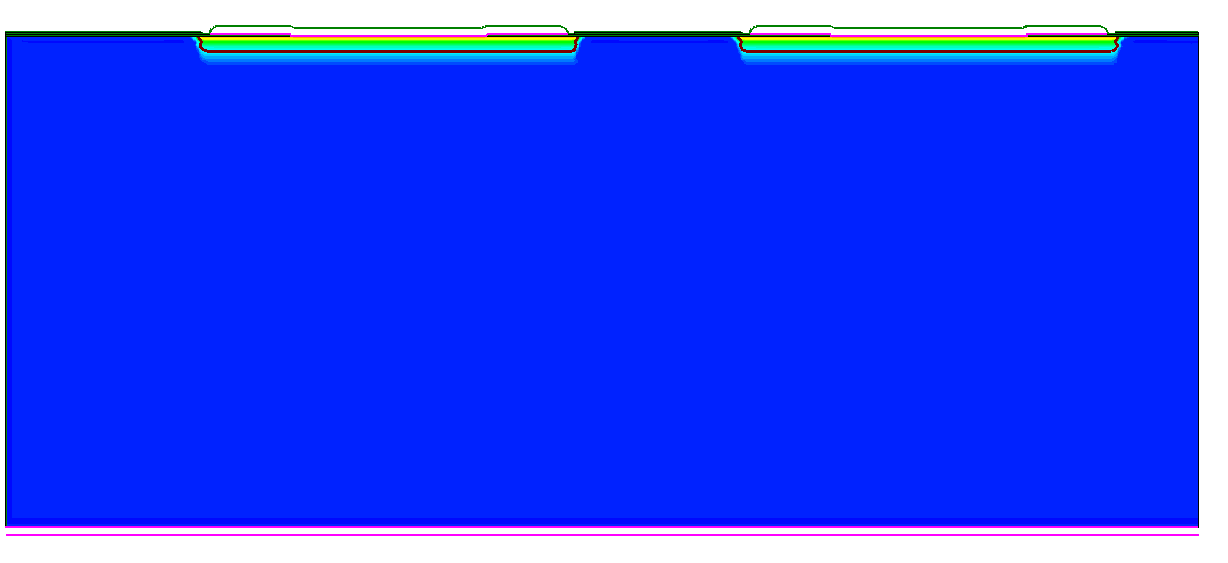
\includegraphics[width=.6\textwidth]{figures/ActiveEdge/schematic.png}};
      \begin{scope}[x={(image.south east)},y={(image.north west)}]
        \draw[-, dashed, line width=.7pt, color=white](0.1, 0.05) -- (0.1, 0.92);
        \draw[-, dashed, line width=.7pt, color=white](0.54, 0.05) -- (0.54, 0.92);
        \draw[<->, line width=.7pt, color=black](0.01, 0.97) -- (0.16, 0.97); % edge width
        
        \node[above, color=black] at (0.05, 0.97) {edge (20 \micron)};
        
        \draw[<->, line width=.4pt, color=black](0.17, 0.97) -- (0.47, 0.97); % n-implant
        \node[above, color=black] at (0.33, 0.97) {n-implant (36 \micron)};
        \node[above, color=white] at (0.3, 0.5) {p-substrate};
        \draw[<->, line width=.4pt, color=black](0.54, 0.0) -- (0.98, 0.0); % pixel width
        \node[below, color=black] at (0.75, 0.0) {pixel (55 \micron)};
        
        \draw[-, line width=3pt, color=violet](0.0, 0.05) -- (0.98, 0.05); % p+ backside contact
        \node[below, color=violet] at (0.15, 0.0) {p+ backside contact};
        \draw[-, line width=3pt, color=violet](0.0, 0.045) -- (0.0, 0.93); % p+ active-edge contact
        \node[left, color=violet, rotate=90] at (-0.05, 0.7) {p+ active edge};
        \node[left, color=white, rotate=90] at (0.08, 0.7) {final pixel edge};

        % \draw[help lines,xstep=.1,ystep=.1] (0, 0) grid (1,1);
        % \foreach \x in {0,1,...,9} { \node [anchor=north] at (\x/10,0) {0.\x}; }
        % \foreach \y in {0,1,...,9} { \node [anchor=east] at (0,\y/10) {0.\y}; }

      \end{scope}
    \end{tikzpicture}
    \caption{Schematic showing the cross section of a sensor with
      $20\,\micron$ active-edge technology. The pixel edges considered
      in the analysis are indicated with dashed lines.}
    \label{fig:activeedge}
  \end{center}
\end{figure}


\begin{table}[htbp]
  \centering
  \caption{Advacam active-edge n-in-p planar pixel sensor assemblies. The edge distance is defined by the distance between the last pixel implant and the physical sensor edge.}
  \label{tab:activeEdgeAssembliesList}
  \begin{tabular}{lccc}
    \toprule
    Assembly & Thickness [\micron] & Edge distance [\micron] & ID \\
    \midrule
    20-NGR  & 50 & 20 & W19\_G7 \\
    23-FGR & 50 & 23 & W19\_F7 \\ \hline
    28-GNDGR & 50 & 28 & W19\_L8 \\
    55-GNDGR & 50 & 55 &W19\_C7 \\
    55-GNDGR-100 & 100 & 55 & W5\_E2  \\ \hline
    55-GNDGR-150 & 150 & 55 & W5\_F1 \\
    \bottomrule
  \end{tabular}
\end{table}

The IV measurement is shown in Figure~\ref{fig:IVmeasurements}.

\begin{figure}[htbp]
  \centering
  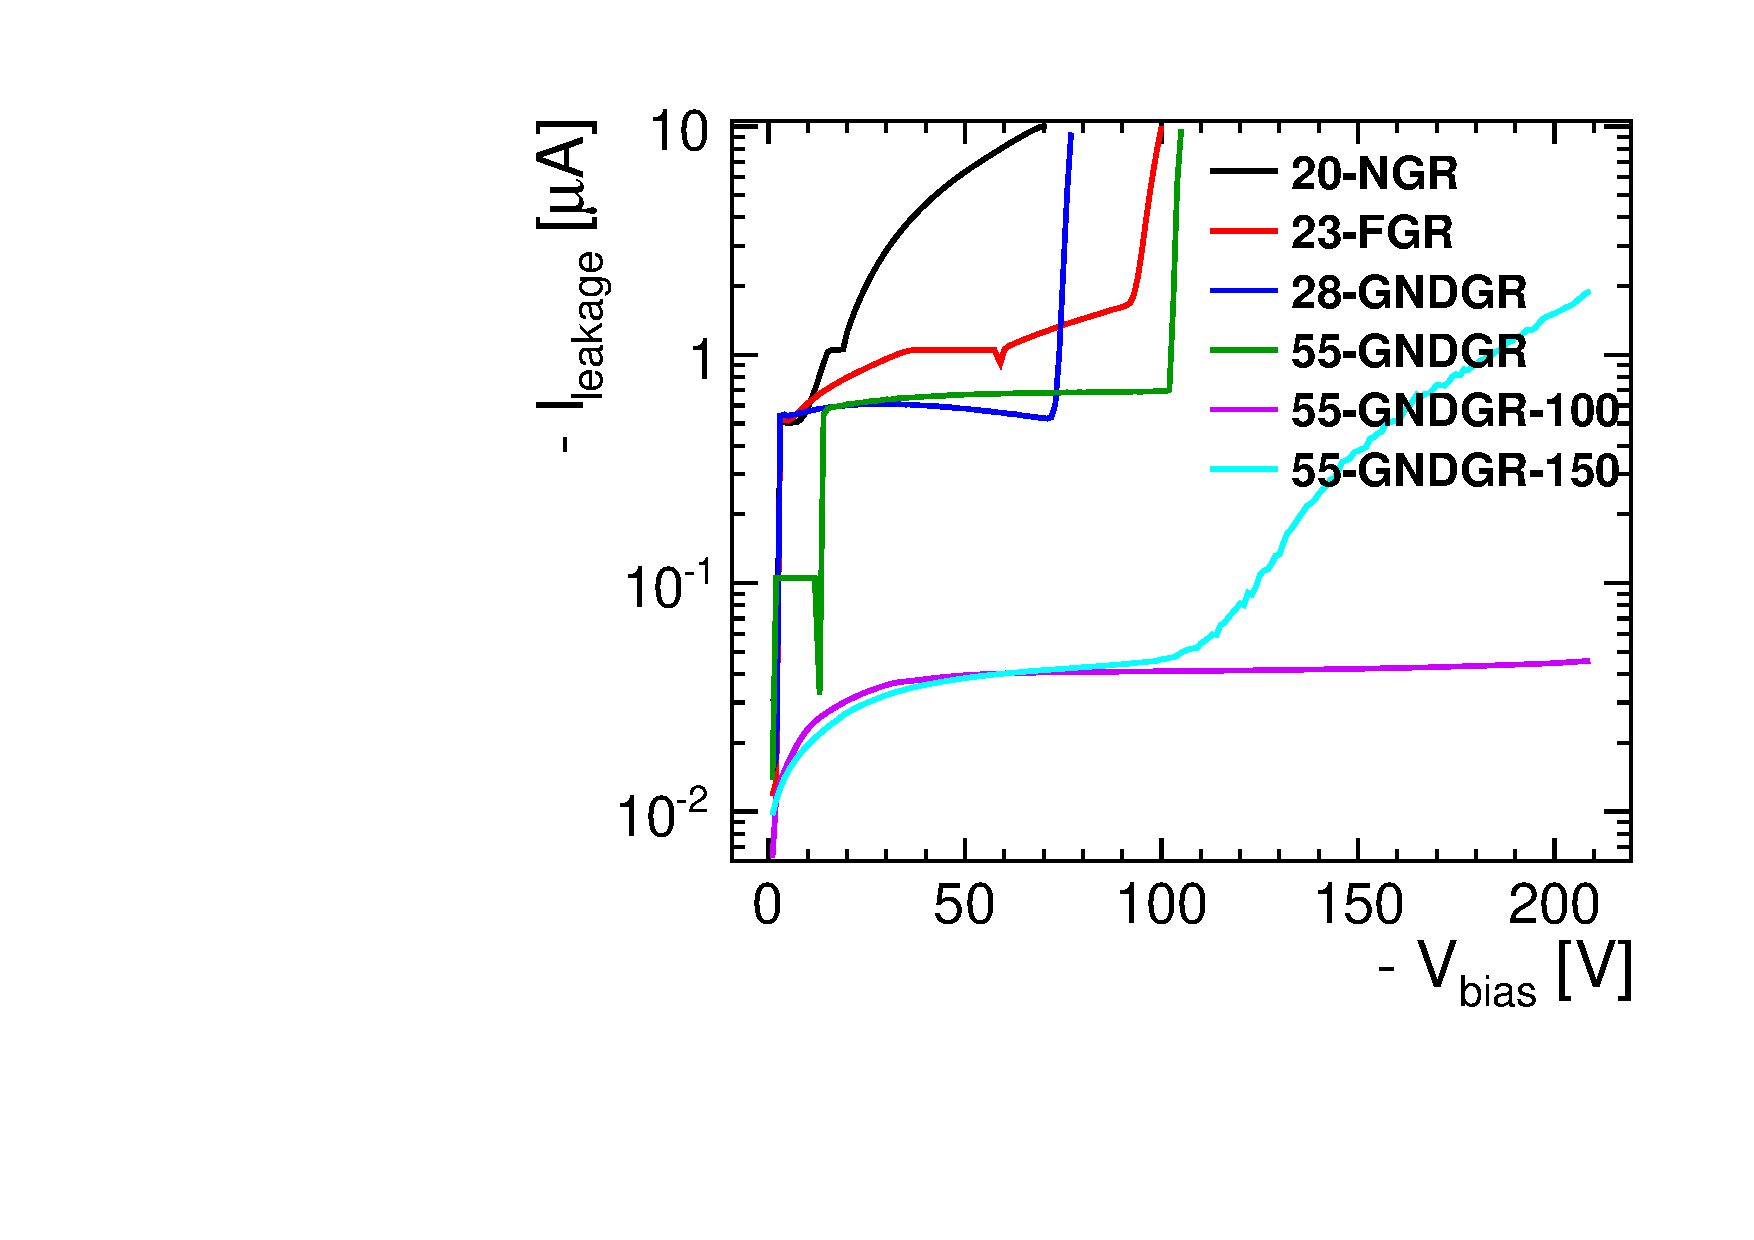
\includegraphics[width=0.7\textwidth]{figures/ActiveEdge/IVCurve.pdf}
  \caption{IV measurements for the assemblies listed in Table~\ref{tab:activeEdgeAssembliesList}.}
  \label{fig:IVmeasurements}
\end{figure}

The layers in the geometry description are defined in
Figure~\ref{fig:PixelLayout} and explained in
Table~\ref{tab:PixelStackDimensions}.

\begin{figure}[htbp]
  \centering
  \begin{minipage}[t]{.4\textwidth}
    \centering
    \vspace{0pt}
    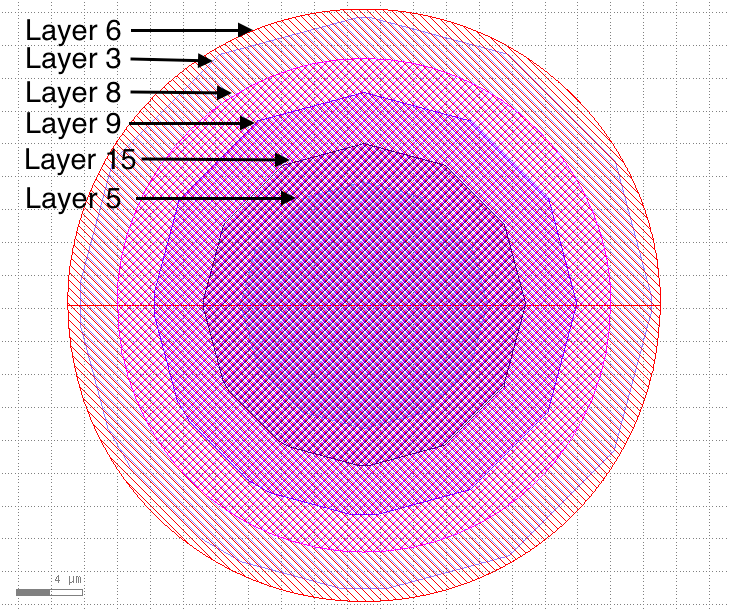
\includegraphics[width=0.95\textwidth]{figures/ActiveEdge/pixelLayout_withLayers.png}
    \caption{}
    \label{fig:PixelLayout}
  \end{minipage}
  \hfill
  \begin{minipage}[t]{.56\textwidth}
    \centering
    \vspace{0pt}
    \captionof{table}{Layers in the sensor from the gds file
      (Picture from 23-FGR).}
    \label{tab:PixelStackDimensions}
    \begin{tabular}{l c c}
      \toprule
      Layer number & Layer \\
      \midrule
      6 & metal\\
      3 & - \\
      8 & implant \\
      9 & UBM (for thin film lift off metal) (??) \\
      15 & passivation \\
      5 & contact to connect Al to Si \\
      \bottomrule
    \end{tabular}
  \end{minipage}
\end{figure}

Table~\ref{tab:DimensionsForAssemblies} summarises the dimensions of
the implants for the sensors. The edge width is the distance between
the last pixel implant to the physical edge of the sensor. The metal
width is the diameter of the metal for the pixels. The doping width is
the diameter of the pixels implant. The contact width is the diameter
of the contact between silicon and the metal (where the oxide is
etched). The GR offset is the distance between the physical edge of
the sensor and the implant of the GR.

\begin{table}
  \centering
  \captionof{table}{The pixels and guard-ring dimensions for different assemblies}
  \label{tab:DimensionsForAssemblies}
  \begin{tabular}{l c c c c}
    \toprule
    & 20-NGR & 23-FGR & 28-GNDGR & 55-GNDGR \\
    \midrule
    Edge width [\micron] & 20 & 23 & 28 & 55 \\
    Metal width [\micron] & 40 & 36 & 36 & 40 \\
    Doping width [\micron] & 30 & 30 & 30 & 30 \\
    Contact width [\micron] & 15 & 15 & 15 & 15 \\
    GR offset [\micron] & - & 10 & 14.5 & 25 \\
    GR doping width [\micron] & - & 5 & 5 & 5 \\
    GR contact width [\micron] & - & 3 & 3 & 15 \\
    GR metal width [\micron] & - & 7 & 7 & 10 \\
    \bottomrule
  \end{tabular}
\end{table}






For the 50~\micron grounded GR, the dimensions of the pixels are
differente from above.
\captionof{table}{Layers and dimensions from the gds geometry
  (taken from Timepix 20um GR FLOAt and from Timepix 50~\micron grounded GR).}
\label{tab:PixelStackDimensions}
\begin{tabular}{l c c c}
  \toprule
  Layer number & Layer & Diameter (20 float) [\micron] & Diameter (50 GND) [\micron]\\
  \midrule
  6 & metal & 36 & 40 \\
  3 & - & 34.62 & 36 \\
  8 & implant & 30 & 30 \\
  9 & UBM & 25.6 & 25.6 \\
  15 & passivation & 19.5 & 19.5 \\
  5 & contact to connect Al to Si & 15 & 15 \\
  \bottomrule
\end{tabular}




\begin{figure}[htbp]
  \centering
  \begin{subfigure}[b]{0.33\textwidth}
    \centering
    \fbox{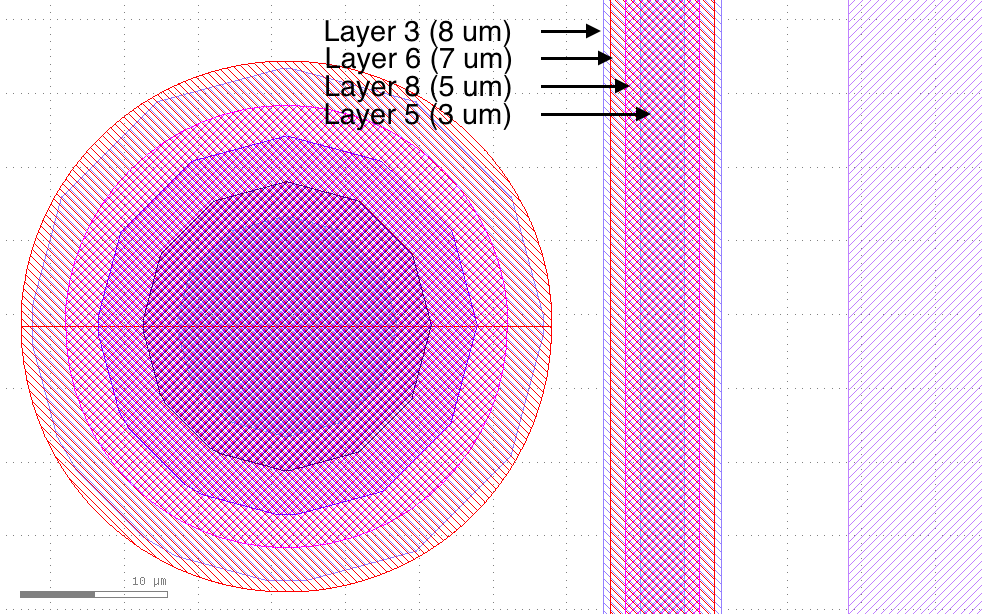
\includegraphics[width=0.95\textwidth]{figures/ActiveEdge/20umEdge_float_GR_withText.png}}
    \caption{20~\micron edge: Floating guard ring}
    \label{fig:GuardRingLayout_20_float_GR}
  \end{subfigure}\hfill
  \centering
  \begin{subfigure}[b]{0.33\textwidth}
    \centering
      \fbox{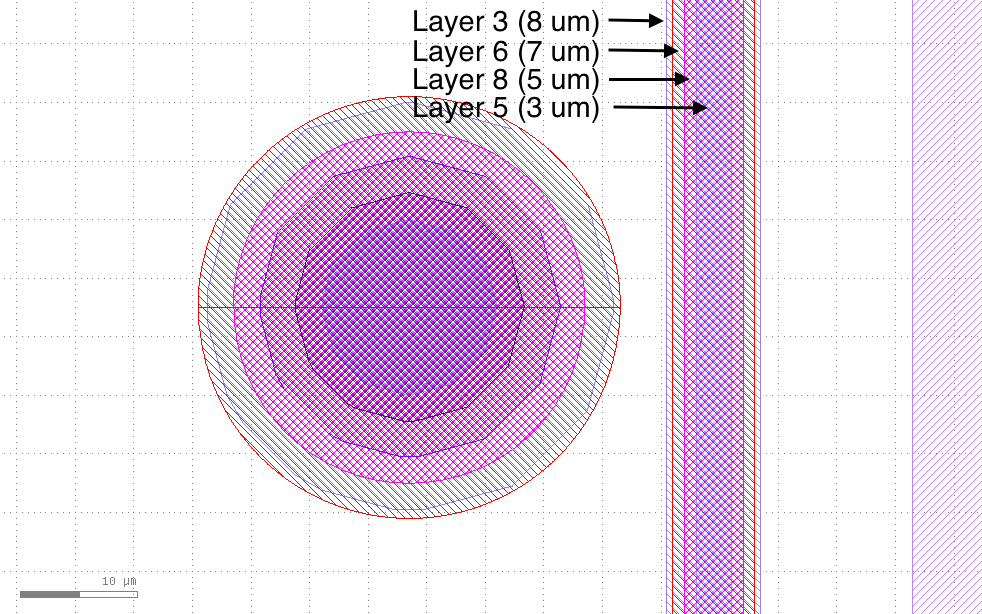
\includegraphics[width=0.95\textwidth]{figures/ActiveEdge/20umEdge_GND_GR_withText.png}}
    \caption{20~\micron edge: GND guard ring}
    \label{fig:GuardRingLayout_20_GND_GR}
  \end{subfigure}\hfill
  \centering
  \begin{subfigure}[b]{0.33\textwidth}
    \centering
    \fbox{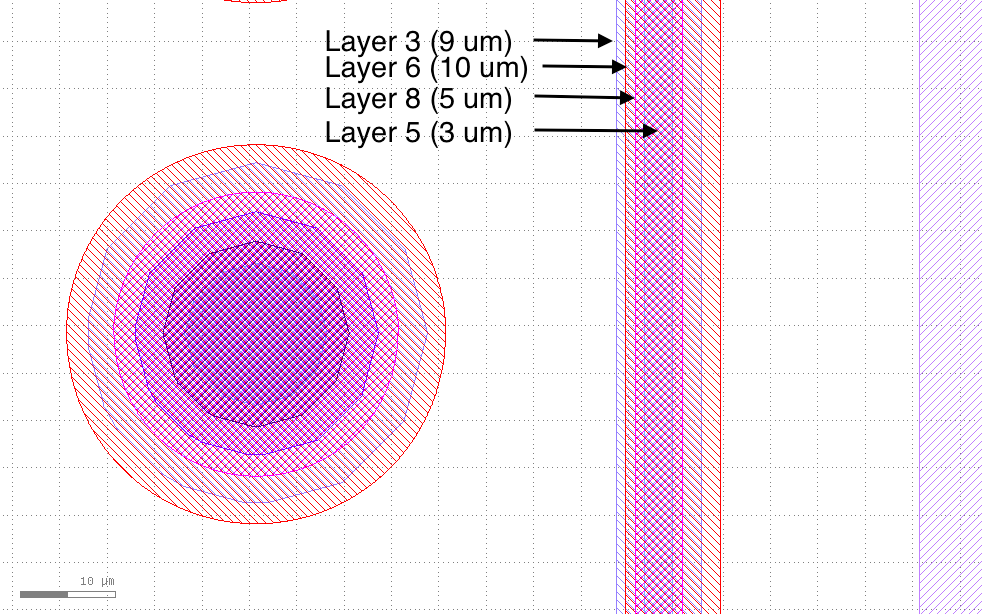
\includegraphics[width=0.95\textwidth]{figures/ActiveEdge/50umEdge_GND_GR_withText.png}}
    \caption{50~\micron edge: GND guard ring}
    \label{fig:GuardRingLayout_50_GND_GR}
  \end{subfigure}
  \label{fig:GuardRingLayout}
\end{figure}

\section{TCAD simulations}

\subsection{Process flow for the active-edge designs}

\begin{itemize}
\item Sprocess 1:
  \begin{enumerate}
  \item First the dimensions of the pixels, implants, contacts, metal
    layer are defined.
  \item The meshing is refined at the borders, the implants and also
    based on the concentration using an adaptive meshing using the
    \texttt{refinebox} command.
  \item The silicon region is then defined for the two pixels and the
    edge region and an extra silicon edge which will be etched (to make
    the process more realistic). The silicon is doped with borons (p-type material)
    with the initial resistivity of $\rho=10000 \Omega$cm. 
  \item A layer of $0.2\,\micron$ thick of Oxide is deposited.
  \item A layer of $0.2\,\micron$ thick of Nitride is deposited.
  \item The silicon is then doped with a concentration of
    $10^{12}\,\inversecmcubic$. From the bias scan of the $150\,\micron$ thick
    silicon, the depletion voltage was obtained at 16~V and confirms the
    doping concentration of the silicon. The implantation done is done
    at the energy of $180\,\kev$.
  \item The nitride is then etched at the positions where the
    implantation is going to be done. First the a mask is put on the
    positions where the Nitride is going to stay. Then the etching is
    done at the implantation positions. Phosphorus (n-type material) is
    implanted with a dose of $10^{15}\,\inversecmcubic$ with an energy
    of $120\,\kev$.
  \item The extra edge is etched to achieve the edge width wanted. First
    the Nitride layer is etched, then the Oxide and finally the silicon
    layer is etched.
  \item The sensor is then flipped and a layer of oxide is deposited on
    the backside with a thickness of $0.04\,\micron$. An implantation is
    done with Boron with a concentration of $10^{15}\,\inversecmcubic$
    with an energy of $60\,\kev$. Then the oxide is etched from the
    backside and the sensor is flipped again to the initial position.
  \end{enumerate}

\item Sprocess 2:
  \begin{enumerate}
  \item The oxide is then etched at the contact positions.
  \item A photoresist is deposited on the top of the sensor with a
thickness of $2\,\micron$.
  \item The meshing of the edge is then refined adaptively depending
on the concentration of the ions and for a thickness of $1\,\micron$.
  \item Borons are implanted to the edge with a concentration of
$10^{15}\,\inversecmcubic$, an energy of $60\,\kev$ and a title of
$15\degrees$C.
  \item The photoresist is then removed (\texttt{strip resist}).
  \item To activate the dopants, the sensor is annealed at a constant
temperature of $940\degrees$C during 240 minutes.
  \item The metal layer is deposited using Aluminium of thickness
$0.8\,\micron$.
  \item The sensor is then flipped and on the back-side, a layer of
aluminium with a thickness of $0.8\,\micron$ for the contact of the
high-voltage is deposited.
  \end{enumerate}
\end{itemize}

Masks limit the etching and the deposition to a certain range of
window and provide the possibility to imitate the lithographic patterning.
% \begin{figure}[htbp]
%   \centering
%   \begin{minipage}[t]{.4\textwidth}
%     \centering
%     \vspace{0pt}
%     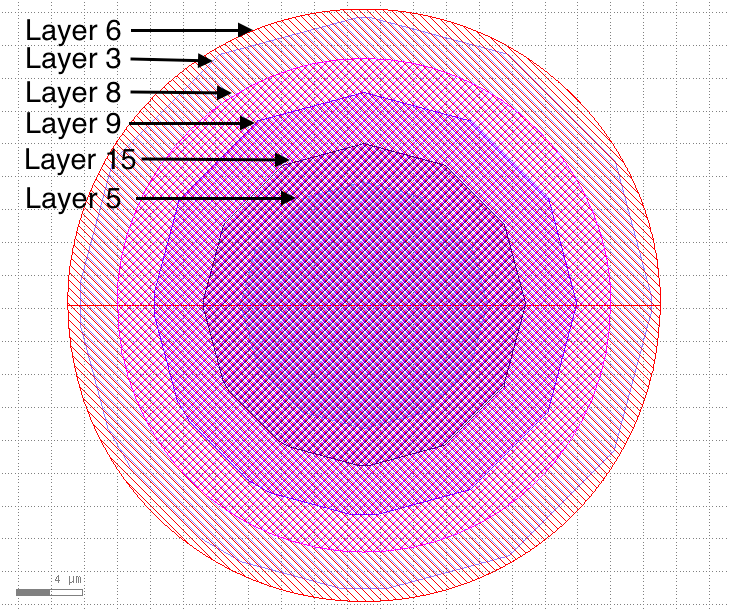
\includegraphics[width=0.95\textwidth]{figures/ActiveEdge/pixelLayout_withLayers.png}
%     \caption{}
%     \label{fig:PixelLayout}
%   \end{minipage}
%   \hfill
%   \begin{minipage}[t]{.56\textwidth}
%     \centering
%     \vspace{0pt}
%     \captionof{table}{Layers and dimensions from the gds geometry
%       (taken from Timepix 20um GR FLOAT).}
%     \label{tab:PixelStackDimensions}
%     \begin{tabular}{l c c}
%       \toprule
%       Layer number & Layer & Diameter [\micron]\\
%       \midrule
%       6 & metal & 36 \\
%       3 & - & 34.62 \\
%       8 & implant & 30 \\
%       9 & UBM (for thin film lift off metal) (??) & 25.6 \\
%       15 & passivation & 19.5 \\
%       5 & contact to connect Al to Si & 15 \\
%       \bottomrule
%     \end{tabular}
%   \end{minipage}
% \end{figure}